\documentclass[a4paper]{extarticle}
\usepackage[utf8]{inputenc}
\usepackage[a4paper, margin=1in]{geometry}

\usepackage{amssymb}
\usepackage{amsmath}
\usepackage{enumitem}
\usepackage{tcolorbox}
\usepackage{fancyhdr}
\usepackage{graphicx}
\usepackage{float}

\setlength{\parindent}{0em}
\setlength{\parskip}{0.4em}

\definecolor{theoremblue}{RGB}{1, 73, 124}
\definecolor{corollaryblue}{RGB}{70, 143, 175}
\definecolor{exampleblue}{RGB}{137, 194, 217}

\newtcolorbox{tbox}{colback=theoremblue!20,colframe=theoremblue,
boxrule=0pt,arc=0pt,boxsep=2pt,left=2pt,right=2pt,leftrule=2pt}

\newtcolorbox{cbox}{colback=corollaryblue!20,colframe=corollaryblue,
boxrule=0pt,arc=0pt,boxsep=2pt,left=2pt,right=2pt,leftrule=2pt}

\newtcolorbox{ebox}{colback=exampleblue!20,colframe=exampleblue,
boxrule=0pt,arc=0pt,boxsep=2pt,left=2pt,right=2pt,leftrule=2pt}

\title{IntroML - Lecture Notes Week 11}
\author{Ruben Schenk, ruben.schenk@inf.ethz.ch}
\date{\today}

\pagestyle{fancy}
\fancyhf{}
\rhead{ruben.schenk@inf.ethz.ch}
\rfoot{Page \thepage}
\lhead{IntroML - Lecture Notes Week 11}

\begin{document}

\maketitle

\subsection{Bayesian Decision Theory}

\subsection{Introduction}

We have seen how we can interpret supervised learning as \textit{fitting probabilistic models} $p(y \, | \, x)$ of the data. Next, we'll see how we can use the estimated models to inform decisions.

Suppose we have estimated a logistic regression model (e.g. for spam filtering), and obtain $p(Y = \text{spam} \, | \, X)$. Furthermore suppose we have three actions: Spam, NotSpam and AskUser.

\textbf{Bayesian decision theory,} a.k.a. maximum expected utility principle, works as follows. Given:

\begin{enumerate}
    \item Conditional distribution over labels $p(y \, | \, x)$ for $y \in Y$
    \item Set of actions $A$
    \item Cost function $C : Y \times A \to \mathbb{R}$
\end{enumerate}

The Bayesian decision theory recommends to pick the action that \textit{minimizes the expected cost:}

\[
    a^* = \arg \min_{a \in \mathcal{A}} \mathbb{E}_y[C(y, \, a) \, | \, x]
\]

If we had access to the true distribution, this decision implements the Bayesian optimal decision (i.e. minimizes the expected cost over all decision rules). In practice, we can only estiamte it, e.g. via logistic regression $p(y \, | \, x)$.

Recall the logistic regression:
\begin{itemize}
    \item \textit{Learning:}
    \begin{align*}
        \hat{w} &= \arg \min_w \sum_{i = 1}^n \log (1 + \exp(-y_iw^Tx_i)) + \lambda ||w||_2^2\\
        &= \arg \max_w P(w \, | \, x_1,..., \, x_n, \, y_1,..., \, y_n)
    \end{align*}
    \item \textit{Classification:}
    \[
        P(y \, | \, x, \, w) = \frac{1}{1 + \exp(-y\hat{w}^Tx)}
    \]
\end{itemize}

\subsection{Optimal Decisions for Classification}

Consider the following setup:
\begin{itemize}
    \item Est. conditional dist.: $p(y \, | x) = \text{Ber}(y; \, \sigma(f(x)))$, e.g. $f(x) = w^Tx$
    \item Action set: $A = \{+1, \, -1\}$
    \item Cost function: $C(y, \, a) = [y \neq a]$
\end{itemize}

Then the action that minimizes the expected cost $a^* = \arg \min_{a \in A} \mathbb{E}_y[C(y, \, a) \, | \, x]$ is the most likely class:

\[
    a^* = \arg \max_y p(y \, | \, x) = \text{sign}(f(x))
\]

\subsection{Asymmetric Costs}

Consider the same setup as above, but with an \textbf{asymmetric cost,} i.e. the cost function is given by:

\[
    C(y, \, a) = \begin{cases}
        c_{FP} &\text{if } y = -1 \text{ and } a = +1\\
        c_{FN} &\text{if } y = +1 \text{ and } a = -1\\
        0 &\text{otherwise}
    \end{cases}
\]

Then the action that minimizes the expected cost $a^* = \arg \min_{a \in A} \mathbb{E}_y[C(y, \, a) \, | \, x]$ is given by the following costs:

\begin{itemize}
    \item $c_+ = \mathbb{E}_y[c(y, \, +1) \, | \, x] = p(y = -1 \, | \, x) \cdot c_{FP} + p(y = +1 \, | \, x) \cdot 0 = (1 - p) \cdot c_{FP}$
    \item $c_- = \mathbb{E}_y[c(y, \, -1) \, | \, x] = p \cdot c_{FN} + (1 - p) \cdot 0 = p \cdot c_{FN}$
\end{itemize}

Therefore, we predict $+1$ if:
\[
    c_+ \leq c_- \Rightarrow (1 - p) \cdot c_{FP} \leq p \cdot c_{FN} \Rightarrow p \geq \frac{c_{FP}}{c_{FP} \cdot c_{FN}}
\]

\subsection{Classification with Abstention}

Consider the same setup as above, but with an \textbf{abstention,} i.e. the action set is given by $A = \{+1, \, -1, \, D\}$ and the cost function by:

\[
    C(y, \, a) = \begin{cases}
        [y \neq a] &\text{if } a \in \{+1, \, -1\}\\
        c &\text{if } a = D
    \end{cases}
\]

Then the action that minimizes the expected cost $a^* = \arg \min_{a \in A} \mathbb{E}_y[C(y, \, a) \, | \, x]$ is given by:

\[
    a^* = \begin{cases}
        y &\text{if } P(y \, | \, x) \geq 1 - c\\
        D &\text{otherwise}
    \end{cases}
\]

In other words, we pick the most likely class only if it's confident enough.

\subsection{Optimal Decisions for LS Regression}

Consider the following setup:
\begin{itemize}
    \item Est. conditional dist.: $p(y, \, | \, x) = \mathcal{N}(y; \, f(x), \, \sigma^2)$, e.g. $f(x) = w^Tx$
    \item Action set: $A = \mathbb{R}$
    \item Cost function: $C(y, \, a) = (y - a)^2$
\end{itemize}

Then the action that minimizes the expected cost $a^* = \arg \min_{a \in A} \mathbb{E}_y[c(y, \, a) \, | \, x]$ is the conditional mean:

\[
    a^* = \mathbb{E}[y \, | \, x] = \int p(y \, | \, x) \, dy = f(x)
\]

\textbf{Example:} We might also consider an asymmetric cost for regression. The setup is the same with a different cost function: $c(y, \, a) = c_1 \max(y - a, \, a) + c_2 \max(a - y, \, 0)$. Then the action that minimizes the expected cost is:

\[
    a^* = f(x) + \sigma \cdot \Phi^{-1}(\frac{c_1}{c_1 + c_2}),
\]

where $\Phi(z) = \int_{- \infty}^{\infty} \mathcal{N}(z; \, 0, \, 1) \, dz$.

\subsection{Active Learning: Uncertainty Sampling}

In general, labels are expensive (since we need to ask an expert). For this reason, we somehow want to minimize the number of labels. One simple strategy is to always pick the example that we are most uncertain about (\textbf{uncertainty sampling}):

Given a pool of unlabeled examples $D_U = \{x_1,..., \, x_n\}$, we also maintain a labeled dataset $D_L$ which is initially empty. For $t = 1, \, 2, \, 3,...$:
\begin{enumerate}
    \item Estimate $p(y \, | \, x)$ given the current data $D_L$
    \item Pick the unlabeled example that we are most uncertain about (highest entropy)
    \[
        i_t \in \arg \min_{x \in D_U} H(p(y \, | \, x))
    \]
    \item Query the label $y_{i_t}$ and set $D_L \leftarrow D_L \cup \{(x_{i_t}, \, y_{i_t})\}$
\end{enumerate}

It is important to note that active learning \textit{violates i.i.d. assumption!} We can get stuck with bad models.

\subsection{Summary}

Bayesian decision theory provides a principled way to derive decision rules from conditional distributions. Standard rules arise as special cases:
\begin{itemize}
    \item Linear regression: $w^Tx$
    \item Logistic regression: $\text{sign}(w^Tx)$
\end{itemize}

Finally, in summary for learning through MAP inference:
\begin{enumerate}
    \item Start with statistical assumptions on data: Data points modeled as i.i.d.
    \item Choose a likelihood function, e.g. Gaussian, student-t, logistic, exponential, etc. This provides the loss function
    \item Choose a prior, e.g. Gaussian, Laplace, etc. This provides the regularizer.
    \item Optimize for MAP parameters
    \item Choose hyperparameters (i.e. variance, etc.) through cross-validation.
    \item Make predictions via Bayesian decision theory
\end{enumerate}

\section{Generative Modeling}

\subsection{Introduction}

Consider the following case:

\begin{figure}[H]
    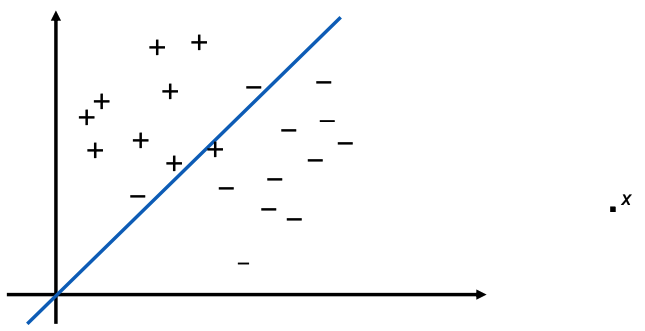
\includegraphics[width=11cm]{../images/IntroML_Fig11-1}
    \centering
\end{figure}

What will logistic regression predict for data point $x$? The problem is that logistic regression can be \textit{overconfident about labels for outliers.}

We can compare discrimiantive and generative models:
\begin{itemize}
    \item \textit{Discriminative models} aim to estimate $p(y \, | \, x)$
    \item \textit{Generative models} aim to estiamte the joint distribution $p(y, \, y)$
\end{itemize}

We can derive a conditional from a joint distribution, but not vice versa!

\subsection{General Approach}

The general approach to \textbf{generative modeling} for classification is:

\begin{itemize}
    \item Estimate prior on labels: $p(y)$
    \item Estimate conditional distribution for each class $y$: $p(x \, | y)$
    \item Obtain predictive distribution using Bayes' rule: $p(y \, | \, x) = \frac{1}{Z}p(y)p(x \, | \, y)$
\end{itemize}

Some notes on generative modeling:
\begin{enumerate}
    \item Generative modeling attempts to infer the process, according tow hich examples are generated
    \item The first generated class label is $p(y)$
    \item Then, generate features given the class $p(x \, | \, y)$
\end{enumerate}

\subsection{Naive Bayes}

For example, we might consider the \textbf{Naive Bayes Model.} In this model, we model class labels as generated from the categorical variable:

\[
    P(Y = y) = p_y \quad y \in \mathcal{Y} = \{1,..., \, c\}
\]

We model features as conditionally independent given $Y$,

\[
    P(X_1,..., \, X_d \, | \, Y) = \prod_{i = 1}^d P(X_1 \, | \, Y),
\]

i.e. given the class label, each features is generated independently of the other features. However, we still need to specify the feature distributions $P(X_i \, | \, Y)$.

In order to predict label $y$ for a new point $x$, we use:

\[
    P(y \, | \, x) = \frac{1}{Z} P(y)P(x \, | \, y) \quad Z = \sum_y P(y)P(x \, | \, y)
\]

\begin{enumerate}
    \item 1. PRedict using Bayesian decision theory.
    \item E.g. in order to minimize misclassification error, we predict:
    \[
        y = \arg \max_{y'} P(y' \, | \, x)
    \]
\end{enumerate}

The \textbf{Gaussian Naive Bayes Classifiers} work as follows. We do the learning given some data $D = \{(x_1, \, y_i),..., \, (x_n, \, y_n)\}$:

\begin{enumerate}
    \item MLE for class prior: $P(Y = y) = \hat{p}_y = \frac{\text{Count}(Y = y)}{n}$
    \item MLE for feature distribution: $P(x_i \, | \, y) = \mathcal{N}(x_i; \, \hat{\mu}_{y, \, i}, \, \sigma^2_{y, \, i})$
    \[
        \hat{\mu}_{y, \, i} = \frac{1}{\text{Count}(Y = y)} \sum_{j;y_j = y}x_{j, \, i}
    \]
    \[
        \sigma^2_{y, \, i} = \frac{1}{\text{Count}(Y = y)} \sum_{j:y_i = y} (x_{j, \, i} - \hat{\mu}_{y, \, i})^2
    \]
\end{enumerate}

Then, the prediction given some new point $x$ is:

\[
    y = \arg \max_y P(y' \, | \, x) = \arg \max_{y'} P(y') \prod_{i = 1}^d P(x_i \, | \, y')
\]

\subsection{Decision Rules for Binary Classification}

We want to predict $y = \arg \max_{y'} P(y' \, | \, x)$. For binary tasks, i.e. $c = 2, \, y \in \{+1, \, -1\}$, this is equivalent to:

\[
    y = \text{sign}\Bigl(\log \frac{P(Y = +1) \, | \, x}{P(Y = -1) \, | \, x}\Bigr)
\]

The function $f(x) = \log \frac{P(Y = +1) \, | \, x}{P(Y = -1) \, | \, x}$ is called \textbf{discriminant function.}

\textbf{Example:} Let us consider the special case of Gaussian Naive Bayes with $c = 2$ and shared variance. We are given $p(x \, | \, y) = \prod_i \mathcal{N}(x_i; \, \mu_{y, \, i}, \, \sigma^2)$. We want $f(x) = \log \frac{P(Y = +1) \, | \, x}{P(Y = -1) \, | \, x}$.

In case of shared variance, GNB produces a linear classifier:

\[
    f(x) = w^Tx + w_0
\]

Hereby:
\[
    w_0 = \log \frac{\hat{p}_+}{1 - \hat{p}_+} + \sum_{i = 1}^d \frac{\hat{\mu}^2_{-, \, i} - \hat{\mu}^2_{+, \, i}}{2 \hat{\sigma}_i^2}
\]
\[
    w_i = \frac{\mu_{+, \, i} - \mu_{-, \, i}}{\sigma_i^2}
\]

The corresponding class distribution

\[
    P(Y = 1 \, | \, x) = \frac{1}{1 + \exp(-f(x))} = \sigma(w^Tx + w_0)
\]

has the \textit{same form as logistic regression.} If model assumptions are met, GNB will make the same predictions as logistic regressions.

Issues with Naive Bayes models:
\begin{itemize}
    \item Conditional independence assumption means that features are generated independently given the class label
    \item If there is conditional correlation between class labels, then this assumption is violated
    \item Due to conditional independence assumption, predictions can become overconfident (very close to 0 or 1)
    \item This might be fine if we care about most likely class only, but not if we want to use probabilities for making decisions (e.g. asymmetric losses etc.)
\end{itemize}

\subsection{Gaussian Bayes Classifiers}

Lets consider general Gaussian Bayes classifiers:
\begin{itemize}
    \item Model class label as generated from categorical variable: $P(Y = y) = p_y$ and $y \in \mathcal{Y} = \{1,..., \, c\}$
    \item Modeal features as generated by multivariate Gaussian: $P(x \, | \, y) = \mathcal{N}(x; \, \mu_y, \, \Sigma_y)$
\end{itemize}

The MLE for Gaussian Bayes classifiers with given data set $D = \{(x_1, \, y_1),..., \, (x_n, \, y_n)\}$ is given by:
\begin{itemize}
    \item MLE for class label distribution
    \[
        P(Y = y) = \hat{p}_y \quad \hat{p}_y = \frac{\text{Count}(Y = y)}{n}
    \]
    \item MLE for feature distribution
    \[
        P(x \, | \, y) = \mathcal{N}(x; \, \hat{\mu}_y, \, \hat{\Sigma}_y)
    \]
    \[
        \hat{\mu}_y = \frac{1}{\text{Count}(Y = y)} \sum_{i:y_i=y} x_i
    \]
    \[
        \hat{\sigma}_y = \frac{1}{\text{Count}(Y = y)} \sum_{i:y_i=y}(x_i \hat{\mu}_y)(x_i - \hat{\mu}_y)^T
    \]
\end{itemize}

\subsection{Fisher's Linear Discriminant Analysis LDA}

Suppose we fix $p = 0.5$ and that the covariances are equal, i.e. $\hat{\Sigma}_- = \hat{\Sigma}_+ = \hat{\Sigma}$. Then the discriminant function simplifies to:

\[
    f(x) = x^T\hat{\Sigma}^{-1}(\hat{\mu}_+ - \hat{\mu}_-) + \frac{1}{2}(\hat{\mu}_-^T \Sigma^{-1}\hat{\mu}_- - \hat{\mu}_+^T \Sigma^{-1}\hat{\mu}_+) = x^Tw + w_0
\]

Under these assumptions, we predict:

\[
    y = \text{sign}(f(x)) = \text{sign}(w^Tx + w_0)
\]

This linear classifier is called \textbf{Fisher's linear discriminant analysis.}

\end{document}